\newpage
\subsection{Kurvenschar}

Eine Kurvenschar ergiebt sich darurch das das $c$ bein intigreieren nicht bestimmt ist: $f(x)dx = F(x)+c$.\\
Und da $c \in \mathbb{R}$ wegeben sich verschiedene Möglichkeiten für $c$ was sin in den möglichen Kurven wiederspiegelt.

\hfill \break
Example:\\
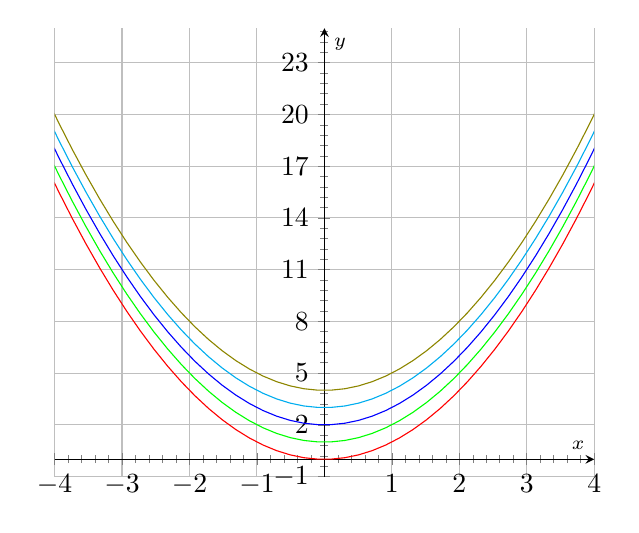
\begin{tikzpicture}[scale=1]
    \begin{axis}%
        [
            grid=major,
            xtick={-5,-4,...,4},
            minor x tick num=4,
            xmin=-4,
            xmax=4,
            xlabel={\scriptsize $x$},
            axis x line=middle,
            ytick={-1,2,...,25},
            minor y tick num=4,
            ymin=-1,
            ymax=25,
            ylabel={\scriptsize $y$},
            axis y line=middle,
            no markers,
            samples=100,
            domain=-10:10,
        ]
        \addplot[red] (x,{x^2+0});
        \addplot[green] (x,{x^2+1});
        \addplot[blue] (x,{x^2+2});
        \addplot[cyan] (x,{x^2+3});
        \addplot[olive] (x,{x^2+4});
    \end{axis}
\end{tikzpicture}